% Provenance (never printed): cycle 4 SVT/physique, "La planete Terre,
% l'environnement": the atmosphere, its structure and its layers, pressure
% and altitude, the ozone layer; see sources/book1/PROVENANCE.md. Book 1,
% grade 8, chapter 1.
% Vocabulary guard: owns the layers of the atmosphere (troposphere,
% tropopause, stratosphere, mesosphere, thermosphere), the environmental
% lapse rate and the ozone layer. Air pressure and the barometer are the
% physics books' (recalled), the composition of air and ozone the molecule
% the chemistry books'; "convection cell" is g8.2's and is not used here;
% adiabatic cooling is Book 2's.
\chapter{A atmosfera}\label{ch:g8:the-atmosphere}

Numa \omterm{def:g4:clouds-rain-snow:weather-station}{estação meteorológica}, pouco antes da hora combinada, uma
meteorologista sai para o gramado segurando um balão cheio de hidrogênio
ou de hélio, com cerca de \qty{1.5}{m} de diâmetro. Embaixo dele, num fio
comprido, ficam pendurados um pequeno paraquedas laranja e uma caixa de
instrumentos de 60 a 80 gramas: uma \emph{radiossonda}. Ela solta o
balão. Ele sobe cerca de \qty{300}{m} por minuto, e a cada segundo a
radiossonda transmite por rádio a pressão, a temperatura, a umidade e a
sua posição. À medida que sobe, o balão incha, até ter de 6 a \qty{8}{m}
de diâmetro e estourar, muitas vezes a mais de \qty{30}{km} de altura,
duas horas depois do lançamento. Nas mesmas horas de todos os dias, a
mesma cena acontece em mais de 800 estações no mundo inteiro.
% ledger: nws:radiosonde

\begin{omfigure}
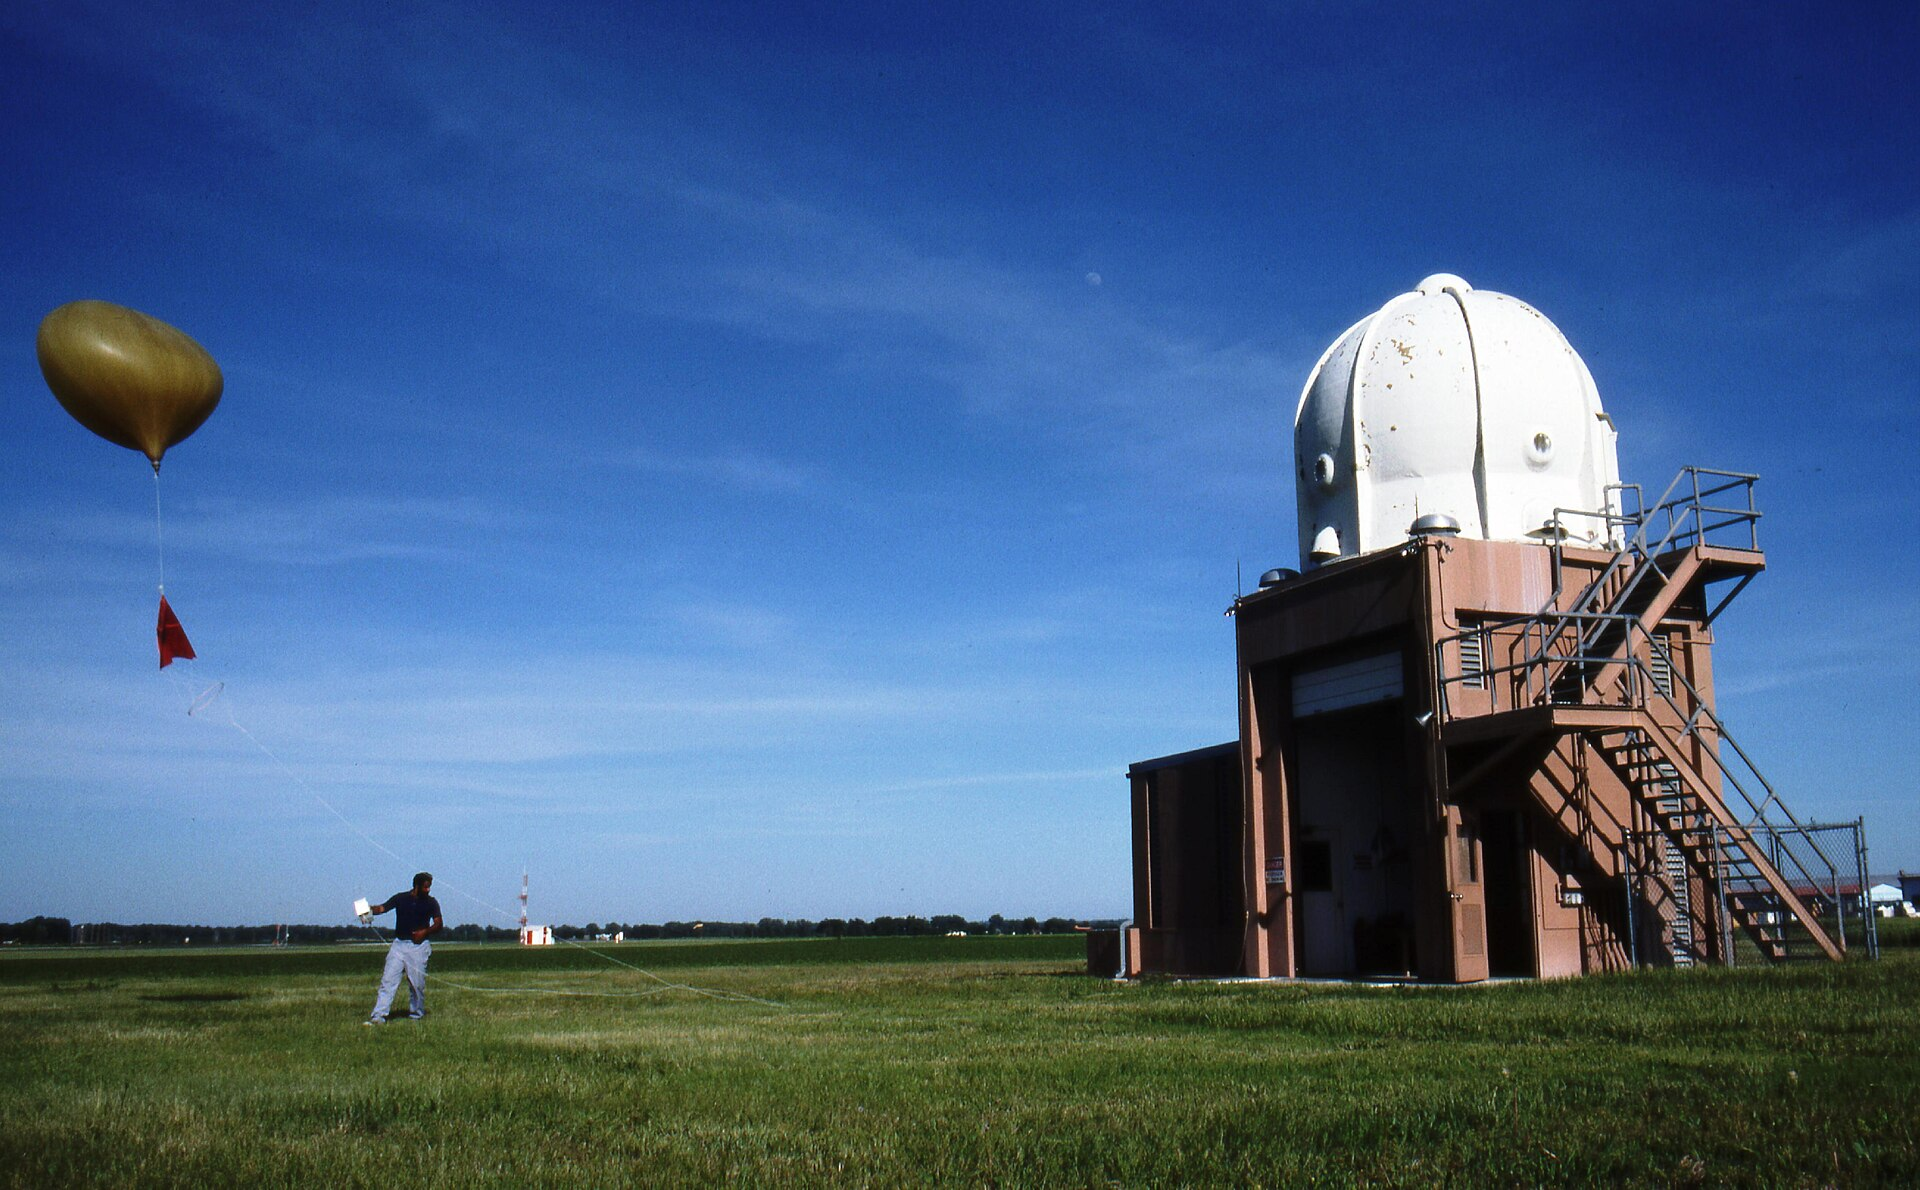
\includegraphics[width=0.78\linewidth]{images/book1/g8-radiosonde-launch.jpg}

{\small Lançamento de um balão meteorológico em Topeka, no Kansas
(Estados Unidos): o paraquedas (vermelho) e a radiossonda ficam
pendurados embaixo do balão. Fotografia de Stephen Corfidi, NOAA/National
Weather Service (domínio público, via Wikimedia Commons).}
% ledger: commons:radiosonde-launch
\label{fig:g8:the-atmosphere:launch}
\end{omfigure}

Por que o balão incha enquanto sobe? O que a radiossonda mede no caminho
para cima, e por que a temperatura não continua simplesmente caindo? Onde
o ar termina?

\begin{recall}
A \emph{atmosfera} é a camada de ar em volta da Terra. O ar faz pressão
sobre tudo o que ele toca: é a \emph{pressão atmosférica}, medida com um
barômetro (os livros de física). Os serviços meteorológicos a dão em
hectopascais (hPa); no \omterm{def:g4:world-physical-map:altitude}{nível do mar}, ela é de cerca de \qty{1013}{hPa}. O
ar seco é feito de cerca de 78~\% de nitrogênio e 21~\% de oxigênio, com
um pouco de argônio, de gás carbônico e de outros gases (os livros de
química). As \omterm{def:g4:clouds-rain-snow:cloud}{nuvens} são feitas de gotinhas de água ou de cristais de gelo
(\cref{ch:g4:clouds-rain-snow}).
\end{recall}
% ledger: air:N2, air:O2, ussa76:sea-level

\section{Um envelope fino}

Vista da Estação Espacial Internacional, a atmosfera é uma linha fina e
luminosa ao longo da borda da Terra. A maior parte do ar, e quase todas as
\omterm{def:g4:clouds-rain-snow:cloud}{nuvens}, estão nos seus poucos quilômetros mais baixos.
% ledger: commons:iss-sunset

\begin{omfigure}
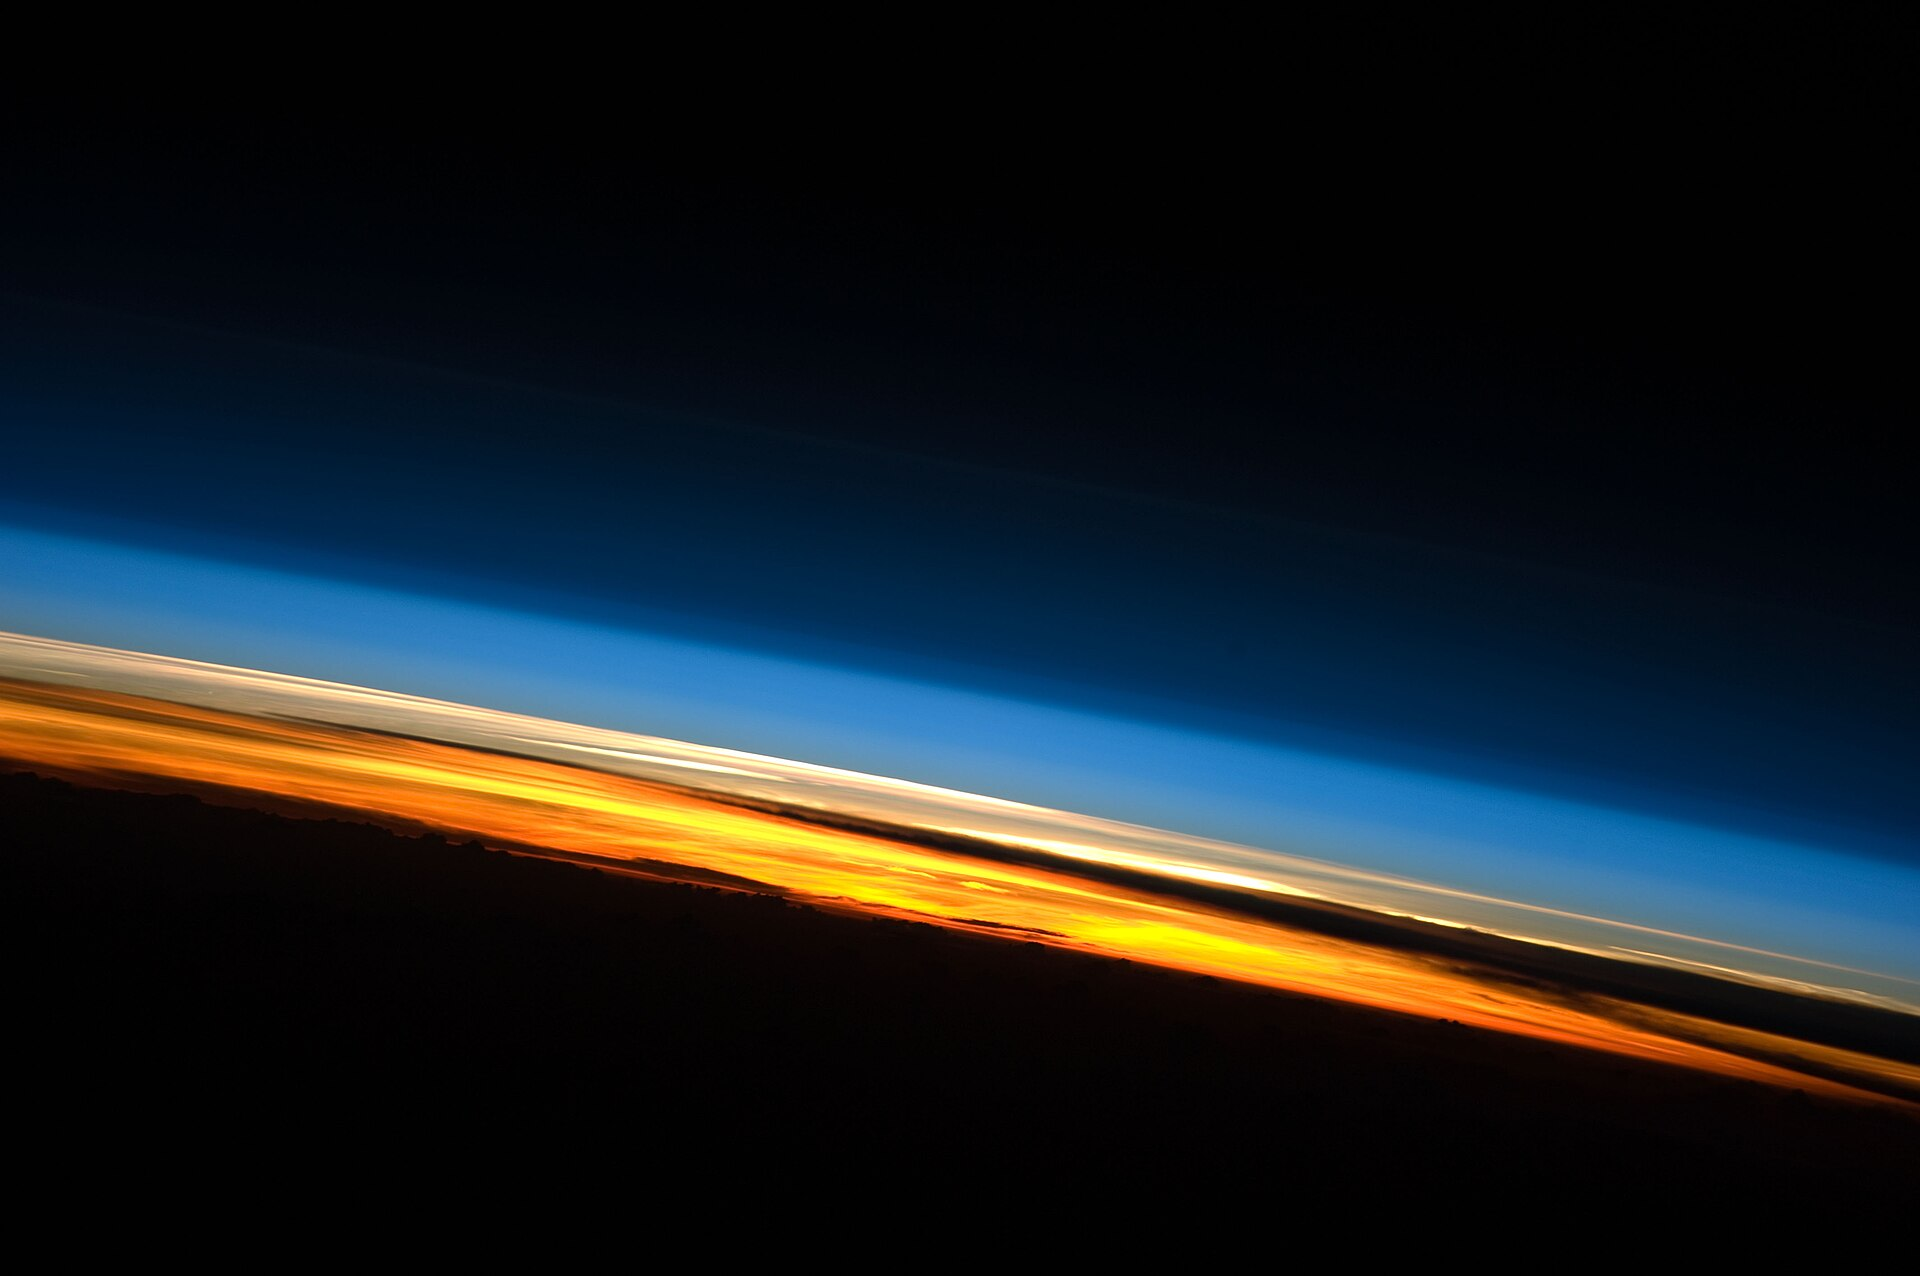
\includegraphics[width=0.78\linewidth]{images/book1/g8-iss-limb.jpg}

{\small A borda da Terra ao pôr do sol, fotografada da Estação Espacial
Internacional acima do \omterm{def:g2:water-on-earth:ocean}{oceano} Índico em 14~de~junho~de~2010. A faixa
laranja e amarela é a camada mais baixa da atmosfera, com as suas \omterm{def:g4:clouds-rain-snow:cloud}{nuvens}
escuras; acima dela vêm camadas mais pálidas e depois azuis, que se
apagam no preto do espaço. Fotografia da NASA, ISS Expedition~23 (domínio
público, via Wikimedia Commons).}
% ledger: commons:iss-sunset
\label{fig:g8:the-atmosphere:limb}
\end{omfigure}

A atmosfera não tem um topo bem definido: o ar fica cada vez mais
rarefeito com a \omterm{def:g4:world-physical-map:altitude}{altitude}. Por convenção, o espaço começa a cerca de
\qty{100}{km}. Em comparação com o raio da Terra, \qty{6371}{km}, isso é
muito pouco: $100 \div
6371 \approx 0.016$, menos de 2~\% do raio. Num \omterm{def:g3:continents-and-oceans:globe}{globo} de \qty{30}{cm} de
diâmetro, a atmosfera inteira seria uma película de cerca de \qty{2}{mm}
de espessura.
% ledger: ucar:layers, earth:Rmean

\begin{omfigure}
\begin{tikzpicture}[font=\footnotesize]
  % 1 cm = 100 km: the Earth's surface is a circle of radius 63.71 cm
  \def\R{63.71}
  \useasboundingbox (-6.9,-1.6) rectangle (6.9,1.0);
  \fill[blue!8] (0,-\R) ++(85:\R+1) arc (85:95:\R+1) -- ($(0,-\R)+(95:\R)$) arc (95:85:\R) -- cycle;
  \fill[omLithAlluv!70] (0,-\R) ++(85:\R) arc (85:95:\R) -- ++(0,-0.6) -- ($(0,-\R)+(85:\R)+(0,-0.6)$) -- cycle;
  \draw[black, line width=0.6pt] (0,-\R) ++(85:\R) arc (85:95:\R);
  \foreach \h/\c in {0.1102/omThm, 0.4938/omMeth, 0.86/omDef} \draw[\c, line width=0.5pt] (0,-\R) ++(85:\R+\h) arc (85:95:\R+\h);
  \draw[black!60, dashed] (0,-\R) ++(85:\R+1) arc (85:95:\R+1);
  \node[anchor=west, omThm] at (5.65,-0.14) {\qty{11}{km}};
  \node[anchor=west, omMeth] at (5.65,0.25) {\qty{49}{km}};
  \node[anchor=west, omDef] at (5.65,0.62) {\qty{86}{km}};
  \node[anchor=east, black!70] at (-5.65,0.75) {\qty{100}{km}};
  \node[anchor=north] at (0,-0.15) {a superfície da Terra};
  \draw[|-|] (-5,-1.05) -- node[below] {\qty{1000}{km}} (5,-1.05);
\end{tikzpicture}

{\small Uma fatia da Terra e da sua atmosfera desenhada em escala
(\qty{1}{cm} para \qty{100}{km}), até \qty{100}{km}, o limite do espaço
(tracejado). As linhas coloridas são os limites das camadas que veremos
mais adiante neste capítulo; a camada mais baixa, onde acontece todo o
\omterm{def:g1:watching-the-weather:weather}{tempo} meteorológico, mal tem um milímetro de espessura.}
% ledger: earth:Rmean, ucar:layers (limits: figdata/grade-8/standard_atmosphere.py main table)
\label{fig:g8:the-atmosphere:to-scale}
\end{omfigure}

\section{A pressão cai com a altitude}

O ar do fundo da atmosfera carrega o peso de todo o ar acima dele. Quanto
mais alto se sobe, menos ar sobra por cima, e mais baixa é a pressão. No
modelo padrão da atmosfera usado pelos meteorologistas e pelos
engenheiros, a pressão é de \qty{1013}{hPa} no \omterm{def:g4:world-physical-map:altitude}{nível do mar}, metade disso
a cerca de \qty{5.5}{km}, e um quarto a cerca de \qty{10.3}{km}.
% ledger: ussa76:sea-level, ussa76:layers (figdata/grade-8/standard_atmosphere.py main table: half_km 5.48, quarter_km 10.29)

Como a pressão mede o peso do ar acima, o nível da meia pressão é também
a altura abaixo da qual fica metade de todo o ar: metade da atmosfera
está espremida nos seus \qty{5.5}{km} mais baixos. Abaixo de \qty{11}{km}
fica cerca de 78~\% do ar; abaixo de \qty{30}{km}, cerca de 99~\%.
% ledger: (computed: figdata/grade-8/standard_atmosphere.py, share_below_11km 77.7, share_below_30km 98.82)

\begin{omfigure}
\begin{minipage}[t]{0.49\linewidth}\centering
\begin{tikzpicture}
\begin{axis}[width=6.6cm, height=7.6cm, xmin=0, xmax=1100, ymin=0, ymax=30,
  xlabel={pressão (hPa)}, ylabel={altitude (km)},
  tick label style={font=\scriptsize}, label style={font=\small},
  xtick={0,250,500,750,1000}, ytick={0,5,10,15,20,25,30}]
  \addplot[dashed, black!60] table {figdata/out/grade-8-standard_atmosphere-guides.dat};
  \addplot[omDef, line width=1.1pt] table[x=p_hPa, y=z_km] {figdata/out/grade-8-standard_atmosphere-pressure.dat};
  \addplot[only marks, mark=*, mark size=1.8pt, omThm, nodes near coords, point meta=explicit symbolic,
    every node near coord/.style={anchor=south west, font=\scriptsize, text=black}]
    table[row sep=\\, x=p_hPa, y=z_km, meta=label] {z_km p_hPa label\\ 5.48 506.6 metade\\ 10.29 253.3 {um quarto}\\ };
\end{axis}
\end{tikzpicture}

{\small A pressão em função da \omterm{def:g4:world-physical-map:altitude}{altitude}. A pressão é a metade do seu valor
no \omterm{def:g4:world-physical-map:altitude}{nível do mar} a cerca de \qty{5.5}{km}, e um quarto a cerca de \qty{10.3}{km}.}
\end{minipage}\hfill
\begin{minipage}[t]{0.49\linewidth}\centering
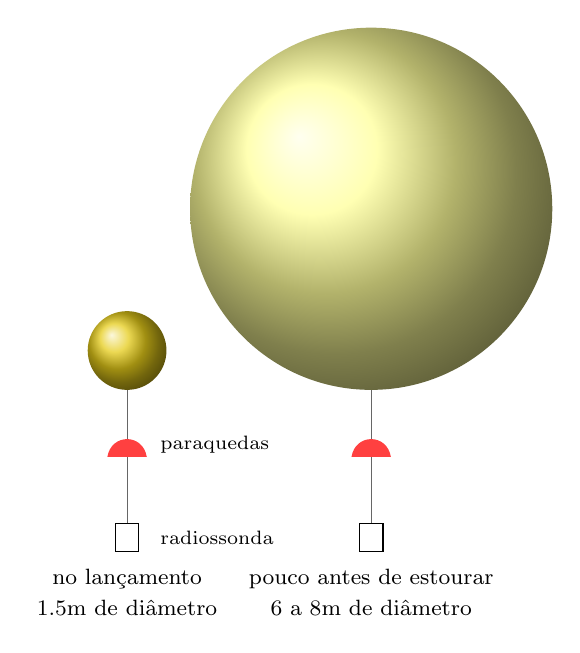
\begin{tikzpicture}[font=\footnotesize]
  % at launch: 1.5 m; at burst: about 7 m (drawn 1 cm for 1.5 m)
  \draw[black!60] (0,0.9) -- (0,2.6);
  \shade[ball color=yellow!60!brown] (0,3.1) circle (0.5);
  \fill[red!75] (-0.25,1.75) .. controls (-0.2,2.05) and (0.2,2.05) .. (0.25,1.75) -- cycle;
  \fill[white, draw=black] (-0.15,0.55) rectangle (0.15,0.9);
  \node[anchor=north] at (0,0.45) {no lançamento};
  \node[anchor=north] at (0,0.05) {\qty{1.5}{m} de diâmetro};
  \begin{scope}[xshift=3.1cm]
    \draw[black!60] (0,0.9) -- (0,2.6);
    \shade[ball color=yellow!40!white] (0,4.9) circle (2.3);
    \fill[red!75] (-0.25,1.75) .. controls (-0.2,2.05) and (0.2,2.05) .. (0.25,1.75) -- cycle;
    \fill[white, draw=black] (-0.15,0.55) rectangle (0.15,0.9);
    \node[anchor=north] at (0,0.45) {pouco antes de estourar};
    \node[anchor=north] at (0,0.05) {6 a \qty{8}{m} de diâmetro};
  \end{scope}
  \node[anchor=west, font=\scriptsize] at (0.3,1.9) {paraquedas};
  \node[anchor=west, font=\scriptsize] at (0.3,0.72) {radiossonda};
\end{tikzpicture}

{\small O balão incha enquanto sobe, porque o ar em volta dele faz cada
vez menos pressão (balões e paraquedas em escala uns com os outros, o fio
encurtado).}
% ledger: nws:radiosonde
\end{minipage}
% ledger: ussa76:sea-level, ussa76:layers (figdata/grade-8/standard_atmosphere.py parts pressure, levels, guides)
\label{fig:g8:the-atmosphere:pressure}
\end{omfigure}

Mais acima, a pressão continua caindo, mais ou menos pela metade de novo a
cada poucos quilômetros, então ela logo fica minúscula. As potências de
dez são a melhor maneira de escrevê-la. A \qty{30}{km}, a pressão é de
cerca de \qty{12}{hPa}, aproximadamente
$10^{-2}$ do seu valor no \omterm{def:g4:world-physical-map:altitude}{nível do mar} (um centésimo); a \qty{50}{km},
cerca de \qty{0.8}{hPa}, aproximadamente $10^{-3}$; a \qty{80}{km}, cerca
de \qty{0.01}{hPa}, aproximadamente $10^{-5}$ da pressão no \omterm{def:g4:world-physical-map:altitude}{nível do mar}.
% ledger: ussa76:layers (figdata/grade-8/standard_atmosphere.py main table: p_30km 11.97, p_50km 0.798, p_80km 0.0105 hPa)

\begin{omfigure}
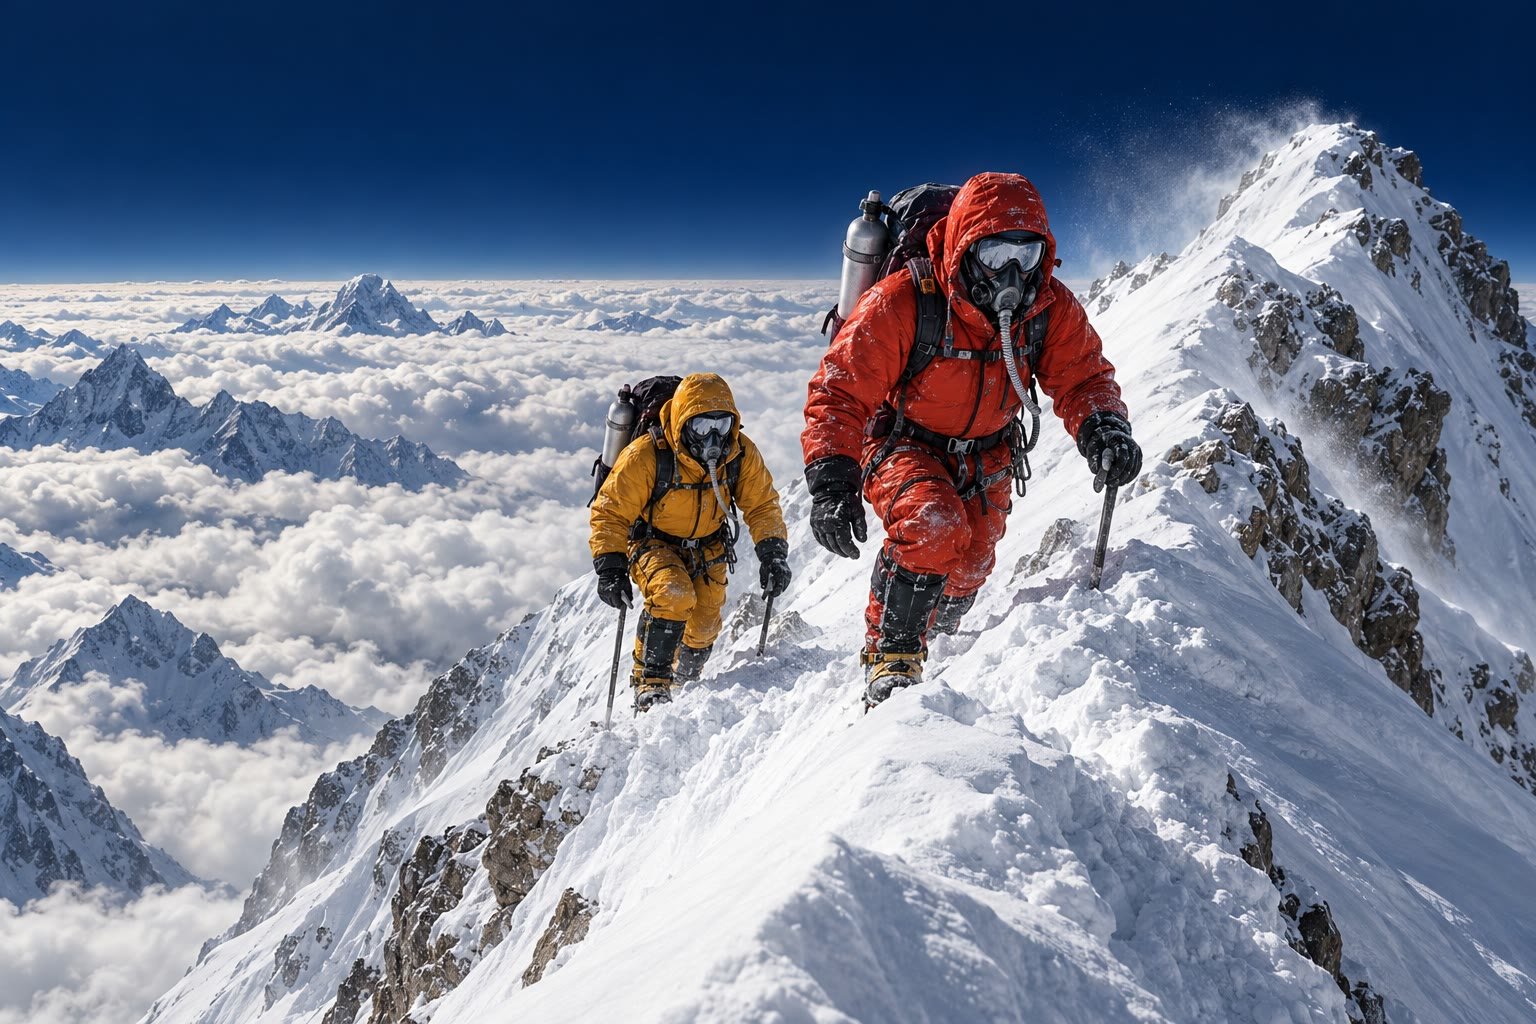
\includegraphics[width=0.5\linewidth]{images/book1/ai/g8-climbers.jpg}

{\small Alpinistas numa \omterm{def:g1:landscapes-around-us:landform}{montanha} muito alta levam garrafas de oxigênio. A
\qty{9}{km}, a pressão é menor que um terço do seu valor no \omterm{def:g4:world-physical-map:altitude}{nível do mar}:
o ar ainda contém 21~\% de oxigênio, mas cada respiração absorve muito
menos dele (ilustração de uma cena genérica feita por IA).}
% ledger: air:O2 (figdata/grade-8/standard_atmosphere.py: pressure at 9 km 308 hPa, 30 % of sea level)
\label{fig:g8:the-atmosphere:climbers}
\end{omfigure}

\section{A temperatura e as camadas}

Todo mundo que já subiu uma \omterm{def:g1:landscapes-around-us:landform}{montanha} sabe que o ar fica mais frio com a
\omterm{def:g4:world-physical-map:altitude}{altitude}. As radiossondas mostram que isso só é verdade na parte mais
baixa da atmosfera. Mais acima, a temperatura para de cair, depois sobe,
depois cai de novo, e depois sobe mais uma vez. Essas mudanças dividem a
atmosfera em camadas.
% ledger: ucar:layers, ussa76:layers

\begin{omfigure}
\begin{tikzpicture}
\begin{axis}[width=10cm, height=9cm, xmin=-100, xmax=30, ymin=0, ymax=100,
  xlabel={temperatura ($^\circ$C)}, ylabel={altitude (km)},
  tick label style={font=\scriptsize}, label style={font=\small},
  xtick={-100,-80,-60,-40,-20,0,20}, ytick={0,10,20,30,40,50,60,70,80,90,100}, axis on top]
  \addplot[fill=omSea!55, draw=none] table {figdata/out/grade-8-standard_atmosphere-band-troposphere.dat};
  \addplot[fill=omMeth!12, draw=none] table {figdata/out/grade-8-standard_atmosphere-band-stratosphere.dat};
  \addplot[fill=omSea!35, draw=none] table {figdata/out/grade-8-standard_atmosphere-band-mesosphere.dat};
  \addplot[fill=omThm!10, draw=none] table {figdata/out/grade-8-standard_atmosphere-band-thermosphere.dat};
  \addplot[omThm, line width=1.2pt] table[x=T_C, y=z_km] {figdata/out/grade-8-standard_atmosphere-temp.dat};
  \addplot[draw=none, nodes near coords, point meta=explicit symbolic,
    every node near coord/.style={anchor=west, font=\small\bfseries, text=black!75}]
    table[row sep=\\, x=lx_C, y=mid_km, meta=name] {name base_km top_km mid_km lx_C\\ troposfera 0 11.02 5.51 -97\\ estratosfera 11.02 49.38 30.2 -97\\ mesosfera 49.38 86 67.69 -97\\ termosfera 86 100 93 -60\\ };
  \draw[black!50, dashed] (axis cs:-100,11.02) -- (axis cs:30,11.02);
  \draw[black!50, dashed] (axis cs:-100,49.38) -- (axis cs:30,49.38);
  \draw[black!50, dashed] (axis cs:-100,86) -- (axis cs:30,86);
  \node[anchor=south east, font=\scriptsize] at (axis cs:17,11.02) {tropopausa};
  \node[anchor=south east, font=\scriptsize] at (axis cs:29,49.38) {estratopausa};
  \node[anchor=south east, font=\scriptsize] at (axis cs:29,86) {mesopausa};
  \fill[omMeth!45] (axis cs:19,16) rectangle (axis cs:23,48);
  \node[anchor=east, font=\scriptsize, align=right] at (axis cs:18,30) {camada\\de ozônio};
\end{axis}
\end{tikzpicture}

{\small A temperatura do ar em função da \omterm{def:g4:world-physical-map:altitude}{altitude}, do chão até
\qty{100}{km}, na atmosfera padrão (uma média para as \omterm{def:g6:latitude-longitude:latitude}{latitudes} médias).
As quatro camadas estão sombreadas; a barra verde marca a altura da
\omterm{def:g8:the-atmosphere:ozone-layer}{camada de ozônio}.}
% ledger: ussa76:sea-level, ussa76:layers, ussa76:above-86, ucar:ozone (figdata/grade-8/standard_atmosphere.py parts temp, layers, band-*)
\label{fig:g8:the-atmosphere:temperature}
\end{omfigure}

\begin{definition}[As camadas da atmosfera]\label{def:g8:the-atmosphere:layers}
De baixo para cima, a atmosfera é dividida em quatro camadas pela maneira
como a sua temperatura muda com a \omterm{def:g4:world-physical-map:altitude}{altitude}:
\begin{itemize}
  \item a \emph{troposfera}\index{troposfera}, onde a temperatura cai com
        a \omterm{def:g4:world-physical-map:altitude}{altitude} e onde acontece quase todo o \omterm{def:g1:watching-the-weather:weather}{tempo} meteorológico; o seu
        topo é a \emph{tropopausa}\index{tropopausa};
  \item a \emph{estratosfera}\index{estratosfera}, onde a temperatura sobe
        com a \omterm{def:g4:world-physical-map:altitude}{altitude}, até cerca de \qty{50}{km};
  \item a \emph{mesosfera}\index{mesosfera}, onde a temperatura cai de
        novo, até cerca de \qty{85}{km};
  \item a \emph{termosfera}\index{termosfera}, onde o ar muito rarefeito
        fica cada vez mais quente com a \omterm{def:g4:world-physical-map:altitude}{altitude}.
\end{itemize}
\end{definition}
% ledger: ucar:layers, ussa76:layers

A \omterm{def:g8:the-atmosphere:layers}{troposfera} contém cerca de 99~\% do vapor de água da atmosfera, então
quase todas as \omterm{def:g4:clouds-rain-snow:cloud}{nuvens}, a \omterm{def:g4:clouds-rain-snow:precipitation}{chuva} e a \omterm{def:g4:clouds-rain-snow:precipitation}{neve} se formam nela. O seu ar é
misturado o tempo todo. O topo da \omterm{def:g8:the-atmosphere:layers}{troposfera} não fica na mesma altura em
todo lugar: a \omterm{def:g8:the-atmosphere:layers}{tropopausa} é mais alta acima do \omterm{def:g3:continents-and-oceans:equator}{equador}, onde pode chegar a
\qty{20}{km}, e mais baixa acima dos \omterm{def:g3:continents-and-oceans:poles}{polos}, onde pode descer a
\qty{7}{km} no inverno. Ela também é mais alta no verão que no inverno.
Na atmosfera padrão, uma média para as \omterm{def:g6:latitude-longitude:latitude}{latitudes} médias, ela fica a
\qty{11}{km}.
% ledger: ucar:layers, ucar:tropopause, ussa76:layers

\begin{definition}[Gradiente térmico vertical]\label{def:g8:the-atmosphere:lapse-rate}
O \emph{gradiente térmico vertical}\index{gradiente termico vertical@gradiente térmico vertical} é o
ritmo em que a temperatura do ar cai com a \omterm{def:g4:world-physical-map:altitude}{altitude} na \omterm{def:g8:the-atmosphere:layers}{troposfera}, em
graus Celsius por quilômetro. Ele muda de um dia para outro e de um lugar
para outro; a atmosfera padrão usa uma média de
\qty{6.5}{\degreeCelsius} por quilômetro.
\end{definition}
% ledger: ussa76:layers

\begin{method}[Ler um perfil de temperatura]\label{met:g8:the-atmosphere:profile}
\begin{enumerate}
  \item Encontre a \omterm{def:g4:world-physical-map:altitude}{altitude} no eixo vertical e vá na horizontal até a
        curva; leia a temperatura embaixo dela.
  \item Onde a curva se inclina para a esquerda ao subir, o ar esfria com
        a \omterm{def:g4:world-physical-map:altitude}{altitude}; onde ela se inclina para a direita, o ar esquenta com
        a \omterm{def:g4:world-physical-map:altitude}{altitude}; onde ela é vertical, a temperatura não muda.
  \item Os limites entre as camadas ficam onde a curva muda de direção.
\end{enumerate}
\end{method}

\begin{example}[Um avião de linha na altitude de cruzeiro]\label{ex:g8:the-atmosphere:airliner}
Um avião de linha voa em cruzeiro a \qty{11}{km}, perto da \omterm{def:g8:the-atmosphere:layers}{tropopausa}. No
perfil, a temperatura ali é de cerca de \qty{-56}{\degreeCelsius}. Com o
gradiente térmico: a partir de \qty{15}{\degreeCelsius} no \omterm{def:g4:world-physical-map:altitude}{nível do mar},
o ar esfria $6.5 \times 11 = 71.5$ graus, o que dá $15 - 71.5 =
\qty{-56.5}{\degreeCelsius}$. Na curva da pressão, a pressão é de cerca
de \qty{227}{hPa}, menos de um quarto da pressão no chão: a cabine
precisa ser pressurizada.
% ledger: ussa76:sea-level, ussa76:layers (figdata/grade-8/standard_atmosphere.py: T at 11 km -56.4 degC, p 227 hPa)
\end{example}

Acima da \omterm{def:g8:the-atmosphere:layers}{tropopausa}, na \omterm{def:g8:the-atmosphere:layers}{estratosfera}, os aviões de linha encontram um voo
mais tranquilo: o ar ali esquenta com a \omterm{def:g4:world-physical-map:altitude}{altitude}, então ele não é
misturado de baixo para cima. Na \omterm{def:g8:the-atmosphere:layers}{mesosfera}, a maioria dos meteoros se
queima, e no seu topo, perto de \qty{86}{km}, fica o ar mais frio de toda
a atmosfera, cerca de \qty{-86}{\degreeCelsius}. Na \omterm{def:g8:the-atmosphere:layers}{termosfera}, os raios X
e a luz ultravioleta do Sol aquecem o ar muito rarefeito a centenas, às
vezes milhares, de graus; mesmo assim, há tão pouco ar que ele não daria
sensação de calor. Muitos satélites giram em volta da Terra ali.
% ledger: ucar:layers, ussa76:above-86

\section{A camada de ozônio}

A \omterm{def:g8:the-atmosphere:layers}{estratosfera} esquenta com a \omterm{def:g4:world-physical-map:altitude}{altitude} porque ela absorve parte da luz do
Sol. O gás que faz a maior parte desse trabalho é o ozônio, uma forma de
oxigênio (a sua química está nos livros de química).

\begin{definition}[Camada de ozônio]\label{def:g8:the-atmosphere:ozone-layer}
A \emph{camada de ozônio}\index{camada de ozonio@camada de ozônio} é a parte da
\omterm{def:g8:the-atmosphere:layers}{estratosfera}, entre cerca de \qty{16}{km} e \qty{48}{km}, onde se
encontra cerca de 90~\% do ozônio da atmosfera. Ela absorve a maior parte
da luz ultravioleta nociva do Sol.
\end{definition}
% ledger: ucar:ozone

Mesmo na \omterm{def:g8:the-atmosphere:ozone-layer}{camada de ozônio}, o ozônio é raro: só de 1 a 10 moléculas em um
milhão. Mesmo assim, junto com o oxigênio, ele barra de 95~\% a 99.9~\%
da luz ultravioleta que chega à Terra, inclusive os tipos mais nocivos. A
energia que ele absorve é transformada em calor, e é por isso que a
temperatura sobe ao longo da \omterm{def:g8:the-atmosphere:layers}{estratosfera}. Sem a \omterm{def:g8:the-atmosphere:ozone-layer}{camada de ozônio}, a luz
ultravioleta que chega ao chão faria mal aos seres vivos.
% ledger: ucar:ozone

\begin{inthefield}[Acompanhar os balões meteorológicos]
Os serviços meteorológicos publicam as medidas das suas radiossondas,
muitas vezes como um gráfico da temperatura em função da \omterm{def:g4:world-physical-map:altitude}{altitude} para
cada lançamento. Com um adulto, procure as sondagens da estação mais perto
de você, feitas às 00:00 ou às 12:00 UTC. Encontre a \omterm{def:g4:world-physical-map:altitude}{altitude} em que a
temperatura para de cair: é a \omterm{def:g8:the-atmosphere:layers}{tropopausa} nesse dia. Compare uma sondagem
de inverno com uma de verão.
\end{inthefield}
% ledger: nws:radiosonde, ucar:tropopause

\section{Exercícios}

\begin{exercise}[$\star$]\label{exo:g8:the-atmosphere:1}
Ligue cada camada à sua descrição: \omterm{def:g8:the-atmosphere:layers}{troposfera}; \omterm{def:g8:the-atmosphere:layers}{estratosfera}; \omterm{def:g8:the-atmosphere:layers}{mesosfera};
\omterm{def:g8:the-atmosphere:layers}{termosfera}. (a) A temperatura sobe com a \omterm{def:g4:world-physical-map:altitude}{altitude} e a \omterm{def:g8:the-atmosphere:ozone-layer}{camada de ozônio}
fica ali. (b) Quase todo o \omterm{def:g1:watching-the-weather:weather}{tempo} meteorológico acontece ali. (c) O ar mais
frio da atmosfera fica no seu topo. (d) O ar muito rarefeito é aquecido a
centenas de graus; muitos satélites giram ali.
\end{exercise}

\begin{exercise}[$\star$]\label{exo:g8:the-atmosphere:2}
Use o perfil de temperatura da atmosfera padrão. (a) Qual é a temperatura
no \omterm{def:g4:world-physical-map:altitude}{nível do mar}? (b) A \qty{11}{km}? (c) A \qty{50}{km}? (d) A
\qty{86}{km}? (e) Entre que \omterm{def:g4:world-physical-map:altitude}{altitudes} a temperatura não muda?
\end{exercise}

\begin{exercise}[$\star$]\label{exo:g8:the-atmosphere:3}
Verdadeiro ou falso? Corrija as frases falsas. (a) A temperatura do ar
sempre cai com a \omterm{def:g4:world-physical-map:altitude}{altitude}. (b) Metade de todo o ar fica abaixo de cerca
de \qty{5.5}{km}. (c) A \omterm{def:g8:the-atmosphere:ozone-layer}{camada de ozônio} fica na \omterm{def:g8:the-atmosphere:layers}{troposfera}. (d) A
\omterm{def:g8:the-atmosphere:layers}{tropopausa} é mais alta acima do \omterm{def:g3:continents-and-oceans:equator}{equador} que acima dos \omterm{def:g3:continents-and-oceans:poles}{polos}.
\end{exercise}

\begin{exercise}[$\star$]\label{exo:g8:the-atmosphere:4}
Em que camada fica cada um destes? (a) Uma \omterm{def:g4:clouds-rain-snow:cloud}{nuvem} de \omterm{def:g4:clouds-rain-snow:precipitation}{chuva}. (b) Um avião
de linha a \qty{12}{km}. (c) Um balão meteorológico pouco antes de
estourar, a \qty{32}{km}. (d) Um meteoro que se queima a \qty{75}{km}.
\end{exercise}

\begin{exercise}[$\star\star$]\label{exo:g8:the-atmosphere:5}
Num dia de verão, faz \qty{20}{\degreeCelsius} no \omterm{def:g4:world-physical-map:altitude}{nível do mar}. Suponha
que o ar esfria \qty{6.5}{\degreeCelsius} por quilômetro. (a) Qual é a
temperatura a \qty{2}{km}? (b) A \qty{3}{km}? (c) A que \omterm{def:g4:world-physical-map:altitude}{altitude},
aproximadamente, o ar chega a \qty{0}{\degreeCelsius}? Arredonde para uma
casa decimal.
\end{exercise}

\begin{exercise}[$\star\star$]\label{exo:g8:the-atmosphere:6}
Um refúgio de \omterm{def:g1:landscapes-around-us:landform}{montanha} fica a \qty{3000}{m}. Uma caminhante sai de uma
aldeia a \qty{500}{m} onde faz \qty{18}{\degreeCelsius}. Usando um
gradiente térmico de \qty{6.5}{\degreeCelsius} por quilômetro: (a) Quantos
quilômetros a caminhante sobe? (b) Quantos graus o ar esfria? (c) Que
temperatura a caminhante pode esperar no refúgio?
\end{exercise}

\begin{exercise}[$\star\star$]\label{exo:g8:the-atmosphere:7}
Suponha que a pressão cai pela metade a cada \qty{5.5}{km}, a partir de
\qty{1000}{hPa} no \omterm{def:g4:world-physical-map:altitude}{nível do mar}. (a) Qual é a pressão a \qty{5.5}{km}? A
\qty{11}{km}? A \qty{16.5}{km}? (b) A atmosfera padrão dá cerca de
\qty{506}{hPa}, \qty{227}{hPa} e \qty{96}{hPa} nessas três \omterm{def:g4:world-physical-map:altitude}{altitudes}
(para \qty{1013}{hPa} no \omterm{def:g4:world-physical-map:altitude}{nível do mar}). A regra da metade é boa perto do
chão? E mais acima?
\end{exercise}

\begin{exercise}[$\star\star$]\label{exo:g8:the-atmosphere:8}
No \omterm{def:g4:world-physical-map:altitude}{nível do mar}, a pressão é de cerca de \qty{1000}{hPa}, ou seja, $10^3$~hPa.
(a) A \qty{30}{km}, ela é de cerca de \qty{10}{hPa}. Escreva isso como uma
potência de dez, e diga quantas vezes ela é menor que no \omterm{def:g4:world-physical-map:altitude}{nível do mar}.
(b) A \qty{80}{km}, ela é de cerca de \qty{0.01}{hPa}. Escreva-a como uma
potência de dez. (c) Quantas vezes ela é menor que no \omterm{def:g4:world-physical-map:altitude}{nível do mar}?
\end{exercise}

\begin{exercise}[$\star\star$]\label{exo:g8:the-atmosphere:9}
Um balão meteorológico tem \qty{1.5}{m} de diâmetro no lançamento e
\qty{6}{m} quando estoura. (a) Quantas vezes mais largo ele fica quando
estoura? (b) Explique por que ele incha enquanto sobe. (c) Por que os
serviços meteorológicos penduram um paraquedas embaixo dele?
\end{exercise}

\begin{exercise}[$\star\star$]\label{exo:g8:the-atmosphere:10}
A \omterm{def:g8:the-atmosphere:layers}{tropopausa} pode chegar a \qty{20}{km} acima do \omterm{def:g3:continents-and-oceans:equator}{equador} e descer a
\qty{7}{km} acima dos \omterm{def:g3:continents-and-oceans:poles}{polos} no inverno. (a) Quantas vezes mais espessa é
a \omterm{def:g8:the-atmosphere:layers}{troposfera} acima do \omterm{def:g3:continents-and-oceans:equator}{equador} nesse caso? Arredonde para uma casa
decimal. (b) No perfil padrão, a \omterm{def:g8:the-atmosphere:layers}{tropopausa} fica a \qty{11}{km}. A
atmosfera padrão está mais perto do \omterm{def:g3:continents-and-oceans:equator}{equador} ou dos \omterm{def:g3:continents-and-oceans:poles}{polos}? (c) Um piloto
voa de uma região polar até o \omterm{def:g3:continents-and-oceans:equator}{equador} a uma \omterm{def:g4:world-physical-map:altitude}{altitude} constante de
\qty{10}{km}. O avião está na \omterm{def:g8:the-atmosphere:layers}{troposfera} ou na \omterm{def:g8:the-atmosphere:layers}{estratosfera} no começo (no
inverno)? E no fim?
\end{exercise}

\begin{exercise}[$\star\star\star$]\label{exo:g8:the-atmosphere:11}
A parte de todo o ar que fica abaixo de uma \omterm{def:g4:world-physical-map:altitude}{altitude} é $1 - p \div
p_0$, onde $p$ é a pressão nessa \omterm{def:g4:world-physical-map:altitude}{altitude} e $p_0 =
\qty{1013}{hPa}$ a pressão no \omterm{def:g4:world-physical-map:altitude}{nível do mar}. (a) A \qty{5.5}{km}, $p
\approx \qty{506}{hPa}$: que parte do ar fica abaixo? (b) A
\qty{11}{km}, $p \approx \qty{227}{hPa}$. (c) A \qty{30}{km}, $p \approx
\qty{12}{hPa}$. Dê as respostas em porcentagem, em números inteiros. (d) Que parte do ar fica acima de \qty{30}{km}?
\end{exercise}

\begin{exercise}[$\star\star\star$]\label{exo:g8:the-atmosphere:12}
Um \omterm{def:g3:continents-and-oceans:globe}{globo} escolar tem \qty{30}{cm} de diâmetro, então o seu raio,
\qty{15}{cm}, representa o raio da Terra, \qty{6371}{km}. (a) Quantos
quilômetros \qty{1}{cm} do \omterm{def:g3:continents-and-oceans:globe}{globo} representa? Arredonde para o quilômetro
mais próximo. (b) Qual seria a espessura, em milímetros, da atmosfera até
\qty{100}{km} nesse \omterm{def:g3:continents-and-oceans:globe}{globo}? (c) E a da \omterm{def:g8:the-atmosphere:layers}{troposfera}, com \qty{11}{km} de
espessura? (d) Uma folha de papel tem cerca de \qty{0.1}{mm} de
espessura. Quantas folhas formariam a \omterm{def:g8:the-atmosphere:layers}{troposfera} do \omterm{def:g3:continents-and-oceans:globe}{globo}?
\end{exercise}

\section{Problema: Acompanhar um balão meteorológico}

\begin{problem}[{Problema de fim de semana --- um balão meteorológico
sobe pela atmosfera; as suas temperaturas mostram as camadas, e as suas
pressões mostram onde sobra um quarto da pressão no nível do mar}]
\label{pb:g8:the-atmosphere:1}
% ledger: nws:radiosonde; the table is the standard atmosphere, figdata/grade-8/standard_atmosphere.py part sonde
Uma radiossonda é lançada de uma estação no \omterm{def:g4:world-physical-map:altitude}{nível do mar}. O seu balão
sobe a cerca de \qty{300}{m} por minuto. A tabela dá a pressão e a
temperatura que ela mede (os valores da atmosfera padrão, arredondados).

\begin{center}\small
\begin{tabular}{|l|*{8}{c|}}
\hline
\omterm{def:g4:world-physical-map:altitude}{altitude} (km) & 0 & 2 & 4 & 6 & 8 & 10 & 12 & 14 \\
\hline
pressão (hPa) & 1013 & 795 & 617 & 472 & 357 & 265 & 194 & 142 \\
\hline
temperatura ($^\circ$C) & 15 & 2 & $-11$ & $-24$ & $-37$ & $-50$ & $-56$ & $-56$ \\
\hline
\hline
\omterm{def:g4:world-physical-map:altitude}{altitude} (km) & 16 & 18 & 20 & 22 & 24 & 26 & 28 & 30 \\
\hline
pressão (hPa) & 104 & 76 & 55 & 40 & 30 & 22 & 16 & 12 \\
\hline
temperatura ($^\circ$C) & $-56$ & $-56$ & $-56$ & $-55$ & $-53$ & $-51$ & $-49$ & $-47$ \\
\hline
\end{tabular}
\end{center}

\noindent\textbf{Parte I --- A subida.}\par\nopagebreak
\begin{enumerate}[beginpenalty=10000]
  \item Quantos metros o balão sobe em 10 minutos?
  \item Quanto tempo ele leva para chegar a \qty{6}{km}? E a \qty{30}{km}?
  \item O balão estoura a \qty{30}{km}. Quanto tempo durou o voo, em
        horas e minutos?
  \item Dê o nome da camada em que o balão está a \qty{8}{km}, e da
        camada em que ele está quando estoura.
\end{enumerate}

\noindent\textbf{Parte II --- A temperatura.}\par\nopagebreak
\begin{enumerate}[resume, beginpenalty=10000]
  \item Quantos graus a temperatura cai entre o chão e \qty{10}{km}?
  \item Qual é o gradiente térmico, em graus por quilômetro, nessa parte
        da subida?
  \item Entre que \omterm{def:g4:world-physical-map:altitude}{altitudes} a temperatura continua a mesma? Onde fica a
        \omterm{def:g8:the-atmosphere:layers}{tropopausa}?
  \item O que acontece com a temperatura acima de \qty{20}{km}? Que gás
        explica isso?
\end{enumerate}

\noindent\textbf{Parte III --- A pressão.}\par\nopagebreak
\begin{enumerate}[resume, beginpenalty=10000]
  \item Quanto é a metade da pressão no \omterm{def:g4:world-physical-map:altitude}{nível do mar}? Entre que \omterm{def:g4:world-physical-map:altitude}{altitudes}
        ela é atingida?
  \item Quanto é um quarto da pressão no \omterm{def:g4:world-physical-map:altitude}{nível do mar}? Arredonde para o
        hectopascal mais próximo.
  \item Entre que duas \omterm{def:g4:world-physical-map:altitude}{altitudes} da tabela esse quarto é atingido?
  \item A pressão cai \qty{71}{hPa} entre \qty{10}{km} e \qty{12}{km}.
        Supondo que ela caia de maneira regular, a que \omterm{def:g4:world-physical-map:altitude}{altitude},
        aproximadamente, a pressão é um quarto do seu valor no \omterm{def:g4:world-physical-map:altitude}{nível do
        mar}? Arredonde para uma casa decimal.
\end{enumerate}
\end{problem}
